%!TEX root = draft.tex
\section{\CRDTLin{}}
\label{sec:distributed-lin}

% \textblue{
% Here we define:
% \begin{itemize}
% \item the notations required for labels: $\aobj.\alabellongind{\argv}{\retv}{i,\ats}$ (partition queries/updates)
% \item the notion of history: $(\alabelset, \avisord)$
% \item the notion of sequential specification: a set of sequences $(\alabelset, \aseqord)$. Talk about per-object specification (and a representation of these specs based on pre/post conditions) and a specification for a set of objects (defined by interleavings)
% \item the notion of \CRDTLin{}: label rewriting + linearization of the visibilities (make it in one shot for both - the intuition should be clear from the overview). Also, in one shot for multiple objects, given that we already defined specifications for multiple objects.
% \item should we talk here about non-determinism and convergence ? (maybe left for later in a discussion section)
% \end{itemize}}

\fxnote[nomargin, inline]{Should we talk here about non-determinism and convergence ? (maybe left for later in a discussion section).}

\fxwarning[nomargin, inline]{MAKE A SUMMARY OF THIS SECTION.}

\subsection{The Semantics of CRDT objects}\label{ssec:semantics}

\fxwarning[nomargin, inline]{MAKE THE CONNECTION WITH THE OVERVIEW. IN PARTICULAR, SAY THAT WE ASSUME CAUSAL DELIVERY, BUT THIS IS ONLY TO SIMPLIFY THE EXPOSITION (AND ANYWAY, IT IS ASSUMED IN MOST IMPLEMENTATIONS)}

\gp{Rewrite?}
The CRDT implementations we consider assume the following two
properties of the propagation of downstreams:
\begin{itemize}
\setlength{\itemsep}{0.5pt}
\item[-] The downstream of each operation is applied exactly once at
  each replica, and
\item[-] If the downstream of operation $\aop_1$ is applied at the
  source replica of $\aop_2$ before $\aop_2$ happens, then for every
  replica $\arep$, the downstream of $\aop_2$ will be applied only
  after the downstream of $\aop_1$ has already been applied.
\end{itemize}
These constraints are commonly guaranteed by network systems
implementing \emph{causal delivery}~\cite{}.

\begin{figure}
\[
  \inferrule[\text{\sc Operation}]
  {\gstates(\arep) = (\alabelset, \astate) \\ \atsource(\sigma,\amethod,\argv) = (\retv,\effector,\ats) \\  \effector(\astate) = \astate' \\ \alabel = \alabelobjind{\argv}{\retv}{(i,\ats)} \\ \mathit{unique}(i) \\
  \ats\neq\bot\implies (\,\forall \alabel\in\alabelset.\ \tsof(\alabel)\neq\bot \implies \tsof(\alabel) < \ats\,) }
  {(\gstates, \avisord, \downstreams) \xrightarrow{\src{\arep}{\alabel}} (\gstates[\arep \leftarrow (\alabelset \cup \{\alabel\}, \astate')], %\alabel
    \avisord \cup (\alabelset \times \{\alabel\}), \downstreams[\alabel \leftarrow \effector])}
\]


\[
  \inferrule[\text{\sc DownStream}]
  {\gstates(\arep) = (\alabelset, \astate) \\ \alabel \in \mathsf{min}_{\avisord}(\labeldom{\avisord} \setminus \alabelset) \\
    \downstreams(\alabel)= \delta \\ \delta(\astate) = \astate'}
  {(\gstates, \avisord, \downstreams) \xrightarrow{\dwn{\arep}{\alabel}} (\gstates[\arep \leftarrow (\alabelset \cup \{\alabel\}, \astate')], \avisord, \downstreams)}
\]

\caption{
  Operational Semantics of CRDTs.
  We use $[A\rightarrow B]$ to denote the set of total functions from
  $A$ to $B$; $C[a \leftarrow b]$ to denote the in-place update of
  element $a$ of the domain of $C$ with value $b$;
  $\mathit{unique}(i)$ to ensure that $i$ is a unique identifier;
  and $\labeldom{\avisord}=\{\alabel: \exists \alabel'.\
  (\alabel,\alabel')\in \avisord \lor (\alabel',\alabel)\in \avisord\}$.
}
\label{fig:crdt-opsem}
\end{figure}


To formalize the semantics of CRDT objects and our correctness
criterion we will introduce the following semantic domains summarized
in~\autoref{fig:sem-dom}.
%
We let $\aobj \in \objs$ be a CRDT object in the set of objects
$\objs$.
Similarly, $\arep \in \reps$ is a replica in the set of replicas
$\reps$.
We assume that both objects and replicas are uniquely identified, and
therefore we will equate an object with its identifier, with the same
convention applying to replicas.

\begin{wrapfigure}{r}{0.5\linewidth}
  \centering
  \(
  \begin{array}[t]{rcll}
    \aobj & \in  & \objs & \text{Objects} \\
    \arep & \in & \reps & \text{Replicas} \\
    \amethod & \in & \methods & \text{Methods}\\
    \argv, \retv & \in & \datadomain & \text{Data Domain} \\
    \ats & \in & \timestampdomain & \text{Timestamp Domain} \\
    % \acrdttyp & \in & \powerset{\methods} \times \powerset{\adomain} & \text{CRDT definition} \\
    % \astate & \in & \states & \text{States} \\
    % \amesg & \in & \messages & \text{Messages} \\
    % \amesgset & \subseteq & \messages & \text{Message Set} \\
    % \aop & \in & \ops \equiv \opids & \text{Operations}\ (ID) \\
    \alabel \equiv \alabelobjind{\argv}{\retv}{i,\ats} & \in & \labels & \text{Operation Label} \\
    \alabelset & \subseteq & \labels & \text{Label Set}\\
    % \arepord & \subseteq & \ops \times \ops & \text{Replica Order} \\
    % \avisord & \subseteq & \ops \times \ops & \text{Visibility Order}
  \end{array}
  \)
  \caption{Semantic Domains.}
  \label{fig:sem-dom}
\end{wrapfigure}


We consider a set of method names $\amethod \in \methods$, and that
each method has a number of arguments sampled from a data domain
$\datadomain$, and a return value also from the data domain.
%
We assume the existence of a special value $\bot \in \datadomain$
which we shall use to represent the absence of a value (for instance
the return type of procedures).
%
We will generally omit writing this value since this value is of no
importance.
%
Furthermore, we ignore here the issues of typing which should be
addressed by an underlying programming language.
Also, some methods, e.g., the method {\tt addAfter} of the RGA object, generate timestamps from a
totally-ordered domain $\timestampdomain$. The order relation on $\timestampdomain$ is denoted by $<$.
%Hence, a data type $\acrdttyp = (\amethodset, \adomain)$ is given by a
%set of method names $\amethodset \subseteq \methods$ and a data domain
%$\adomain \subseteq \datadomain$.

%The timestamp of such an operation label $\alabel$
% We may omit the object $\aobj$ when it is understood from the context.
We will use operation labels of the form
$\alabelobjind{\argv}{\retv}{i,\ats}$ to represent the call of a
method $\amethod \in \methods$ of object $\aobj\in \objs$, with
argument $\argv \in \datadomain$, resulting in the value $\retv \in
\datadomain$, and generating the timestamp $\ats$.
Abusing our notations, we assume that the set $\timestampdomain$
contains a distinguished element $\bot$ which we shall use for
operations that do not generate a timestamp as the method {\tt remove}
of the RGA.
In that case the meta-variable $\ats$ adopts the value $\bot$. We extend the order
relation $<$ on timestamps to include $\bot$ as a minimal element.
The timestamp $\ats$ of an operation label $\alabel=\alabelobjind{\argv}{\retv}{i,\ats}$
is denoted by $\tsof(\alabel)$.
We may omit the object $\aobj$, the timestamp $\ats$, or the return
value when these are not important.
%We assume that in a history all labels are unique.
Since there might be multiple calls to the same method with the same
arguments and result, labels are tagged with a unique identifier $i$.
%as in $\alabellongind{\argv}{\retv}{i}$.
However, since we assume that each label of an operation in an
execution is tagged with a unique identifier, we will ignore
identifiers when unambiguous.
The set of all operation labels is denoted by $\labels$.
%\labels
% the transitions are labeled by operation labels in $\labels$,
%\times \labels

% \gpnote[inline, nomargin]{I would probably state it as a function
%   directly.}
Given a CRDT object $\aobj$, its semantics is defined as a labeled transition
system (LTS) $\llbracket \aobj \rrbracket =
(\globalstates,\acts,\aglobalstate_0,\rightarrow)$ as shown in
\figurename~\ref{fig:crdt-opsem}, where $\globalstates$ is a set of
global configurations, $\acts$ is the set of transition labels called \emph{actions},
$\aglobalstate_0$ is the initial configuration, and
$\rightarrow\subseteq \globalstates \times \acts\times \globalstates$ is the
transition relation. For readability, we use $\aglobalstate \xrightarrow{\aact} \aglobalstate'$
to denote a transition $(\aglobalstate,\aact,\aglobalstate')\in\,\rightarrow$.

A global configuration $(\gstates, \avisord, \downstreams)$ is a
``snapshot'' of the system that records all the operations that have
been executed.
$\gstates \in [\reps \rightarrow \localstates]$ stores the local
configuration of each replica.
A local configuration $(\alabelset, \astate)$ contains the state
$\astate$ of a replica and the set $\alabelset$ of labels of
operations that have been originated at this replica, or whose
downstreams have been executed (or applied) at this replica.
When $\alabel\in \alabelset$, we say that $\alabel$ is \emph{visible}
to the replica or that the replica \emph{sees} $\alabel$.
The relation $\avisord\subseteq \powerset{\labels \times \labels}$ is
the \emph{visibility} relation between operations, i.e.,
$(\alabel_1,\alabel_2)\in \avisord$, where $\alabel_2$ is an operation
originated at a replica $\arep$, if the downstream of $\alabel_1$ was
executed at $\arep$ before $\alabel_2$ was executed.
When $(\alabel_1,\alabel_2)\in \avisord$, we say that $\alabel_1$ is
\emph{visible} to $\alabel_2$, or that $\alabel_2$ \emph{sees}
$\alabel_1$.
As it will be clear from the definition of the transition relation,
$\avisord$ is a \emph{strict partial order} (i.e.
irreflexive and transitive).
Finally, $\downstreams\in [\labels \rightarrow \Delta]$ associates to
each operation label $\alabel \in \alabelset$ a downstream
$\effector\in [\states \rightarrow \states]$, which is the replica
state transformer generated when the operation was executed at the
source replica.

For some fixed initial replica state $\astate_0$, the initial global configuration is defined by $\aglobalstate_0 = (\gstates_0, \emptyset, \emptyset) \in \globalstates$, where $\gstates_0$ maps each replica $\arep$ into $(\emptyset, \astate_0)$.

%\fxwarning[nomargin, inline]{ADD CONSTRAINT ON TIMESTAMPS: THAT THEY INCREASE ACCORDING TO THE VISIBILITY. NEED TO INTRODUCE SOMEWHERE THE ORDER RELATION ON TIMESTAMPS.}

The transition relation between global configurations is defined in
\figurename~\ref{fig:crdt-opsem}.
The first rule describes a replica $\arep$ in state $\astate$
executing an invocation of method $\amethod$ with argument $\argv$.
This transition first applies the {\tt atSource} function $\atsource$
in the state of the source replica, and as a result it outputs a
return value $\retv$, a downstream state transformer $\effector$
to be applied on all replicas, and possibly, a timestamp $\ats$.
As mentioned above, $\ats=\bot$ for methods that don't generate
timestamps. This transition is labeled by an action $\src{\arep}{\alabel}$ where
$\alabel$ is the label of this invocation. We may ignore the index $\arep$ when it is not important.
We assume that timestamps are consistent with the visibility relation
$\avisord$, i.e., the timestamp $\ats$ generated by $\atsource$ is strictly bigger than
all the timestamps of operations visible to $\arep$. Formally, if $\ats\neq\bot$ then $\ats' < \ats$ for all timestamps
$\ats'\neq\bot$ of operations in $\alabelset$.
The association between the label $\alabel$ corresponding to this
invocation and the downstream $\effector$ is recorded in the
$\downstreams$ component of the new global configuration.
We say that the effector $\effector$ is \emph{produced} by the operation $\alabel$.
The local configuration $(\alabelset,\sigma)$ of $\arep$ is changed by
applying the downstream $\effector$ on the state $\sigma$, resulting
in a new state $\sigma'$, and adding $\alabel$ to the set of labels
$\alabelset$.
Finally, the visibility relation $\avisord$ is changed to record the
fact that the downstreams of all operations in $\alabelset$ have been
applied before $\alabel$.
%
\autoref{fig:rga-sem} shows how some components of the semantics
progress according to the rules of~\autoref{fig:crdt-opsem} for the
RGA data type.
%
In particular we shown: the local labels of replica $\arep_1$
($\gstates(\arep_1).\alabelset$); its state, where we remove the
$\astate$ for succinctness (then $\gstates(\arep_1).\astate.\mathsf{N}$
becomes $\gstates(\arep_1).\mathsf{N}$); and the global visibility
relation $\gstates.\mathtt{vis}$.
%
The transition from~\autoref{fig:rga-sem-2} to~\autoref{fig:rga-sem-3}
shows an {\sc Operation} transition where the operation
$\mathtt{remove}(b)$ is executed by replica $\arep_1$.
%
Notice in particular how the global visibility relation is extended.

% \fxwarning[nomargin, inline]{EXAMPLE BASED ON RGA} {\color {red} CW: See the process from \figurename~\ref{fig:an example run of semantics} (b) to \figurename~\ref{fig:an example run of semantics} (c).}

The second rule describes a replica $\arep$ in state $\astate$
executing the downstream $\effector$ that corresponds to an operation
$\alabel$ originated in a different replica.\footnote{We could
  simplify the first rule by not performing the downstream immediately,
  but in general we assume no interleavings of operations within a
  single replica.}
The rule requires that $\effector$ is a downstream of a label that has
not yet been applied at $\arep$ (i.e., its corresponding label is not
in the $\alabelset$ component of $\arep$'s configuration) and
moreover, that it is a minimal one with respect to the order
$\avisord$ among such downstreams, i.e., there exists no
$\alabel'\not\in \alabelset$ such that $(\alabel',\alabel)\in
\avisord$.
This transition, labeled by the action $\dwn{\arep}{\alabel}$ (we may
ignore the index $\arep$ when it is not important), results in
modifying the state of $\arep$ to $\effector(\sigma)$ and adding
$\alabel$ to the set of operations whose downstreams have been
executed by $\arep$.
Remark that these transition rules preserve the fact that $\avisord$
is a strict partial order.
%
In~\autoref{fig:rga-sem}, the transition from~\autoref{fig:rga-sem-1}
to~\autoref{fig:rga-sem-2} corresponds to a {\sc DownStream}
transition which extends the visibility of the operation
$\mathtt{addAfter}(b, d)$ to $\arep_1$.
%
Notice that this is reflected in the $\gstates(\arep_1).\alabelset$
component.
%
The relation $\gstates.\mathtt{vis}$ does not change since this
relation only changes when a new operation is executed at the source
replica.


% \fxwarning[nomargin, inline]{EXAMPLE BASED ON RGA} {\color {red} CW: See the process from \figurename~\ref{fig:an example run of semantics} (a) to \figurename~\ref{fig:an example run of semantics} (b).}

\begin{figure}[t]
  % \centering
  \begin{subfigure}[!ht]{.3\linewidth}
    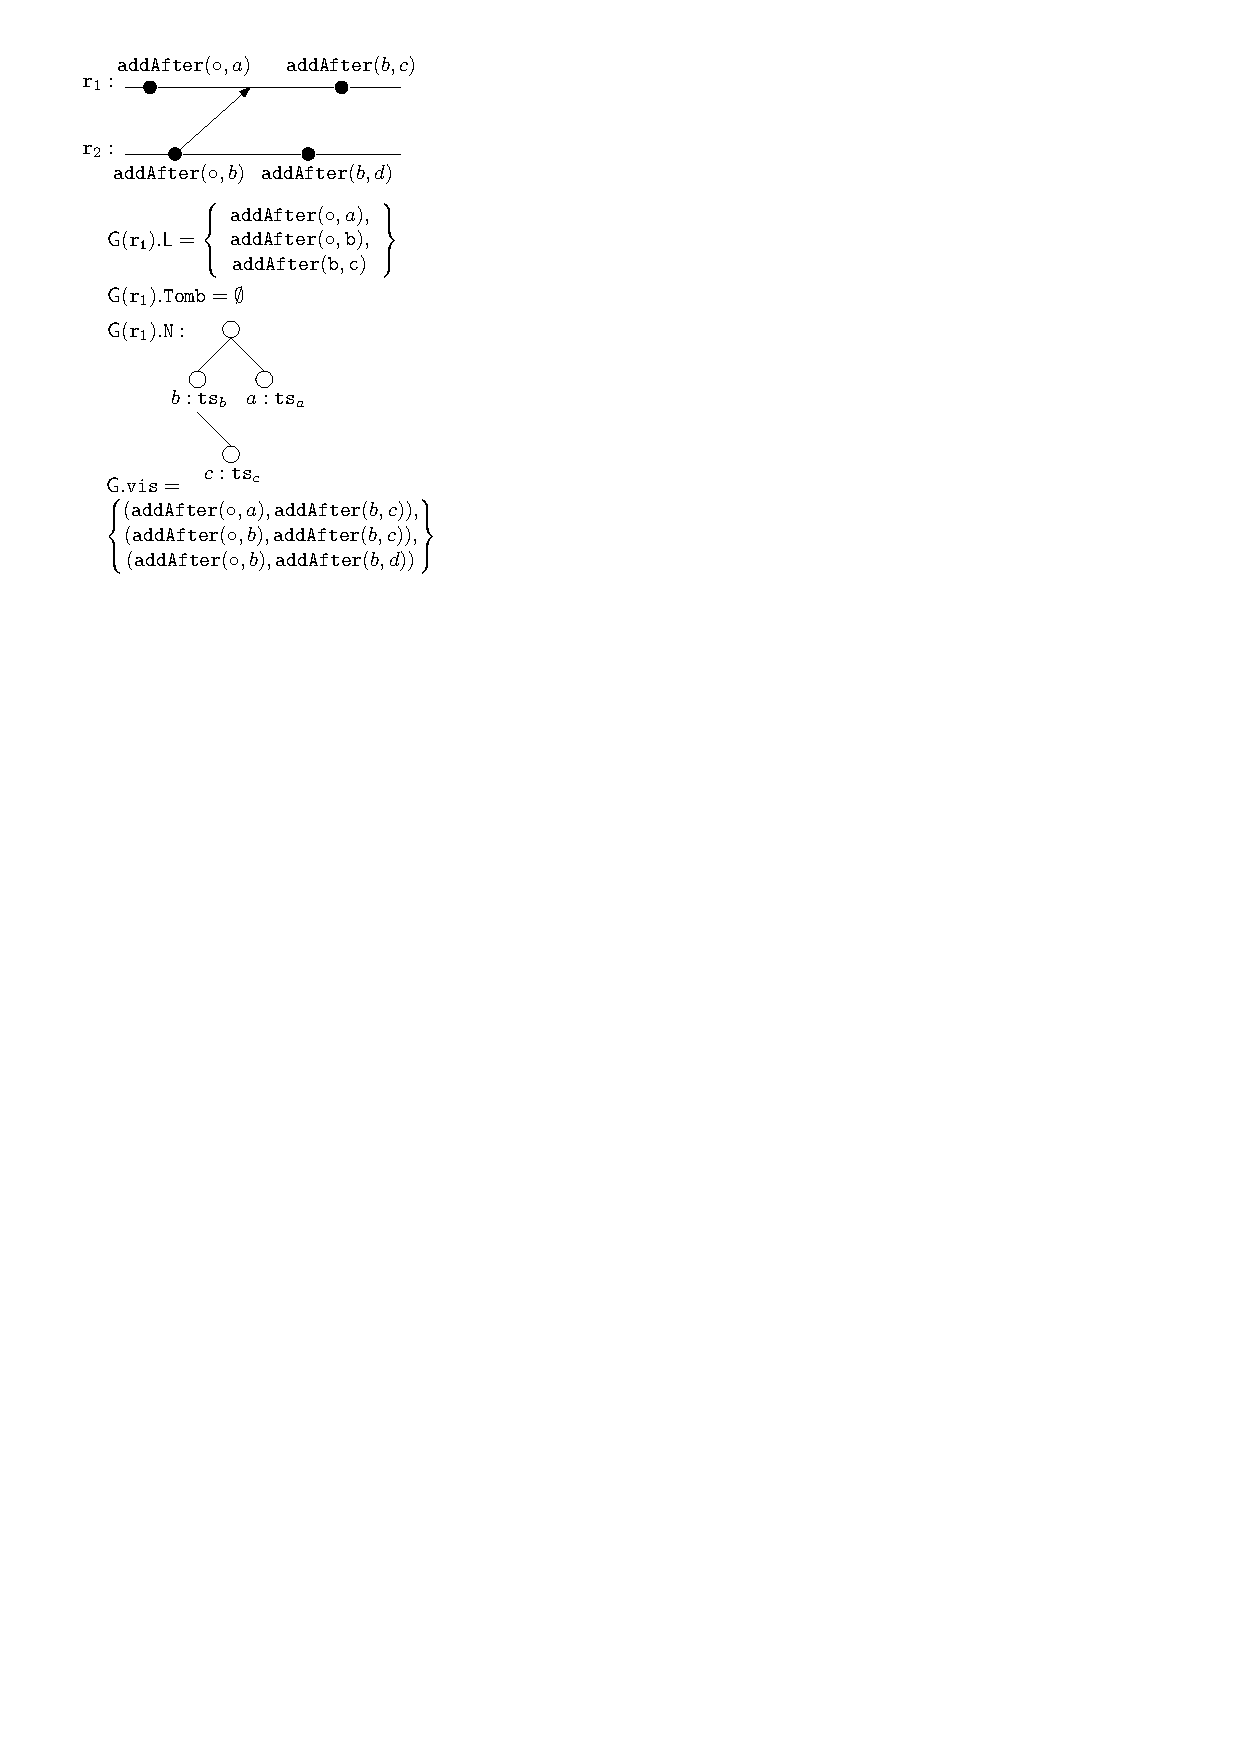
\includegraphics[scale=.7]{figures/LinRGA-1}
      \vspace{1.3cm}
    \caption{}
    \label{fig:rga-sem-1}
  \end{subfigure}
  \begin{subfigure}[!ht]{.3\linewidth}
      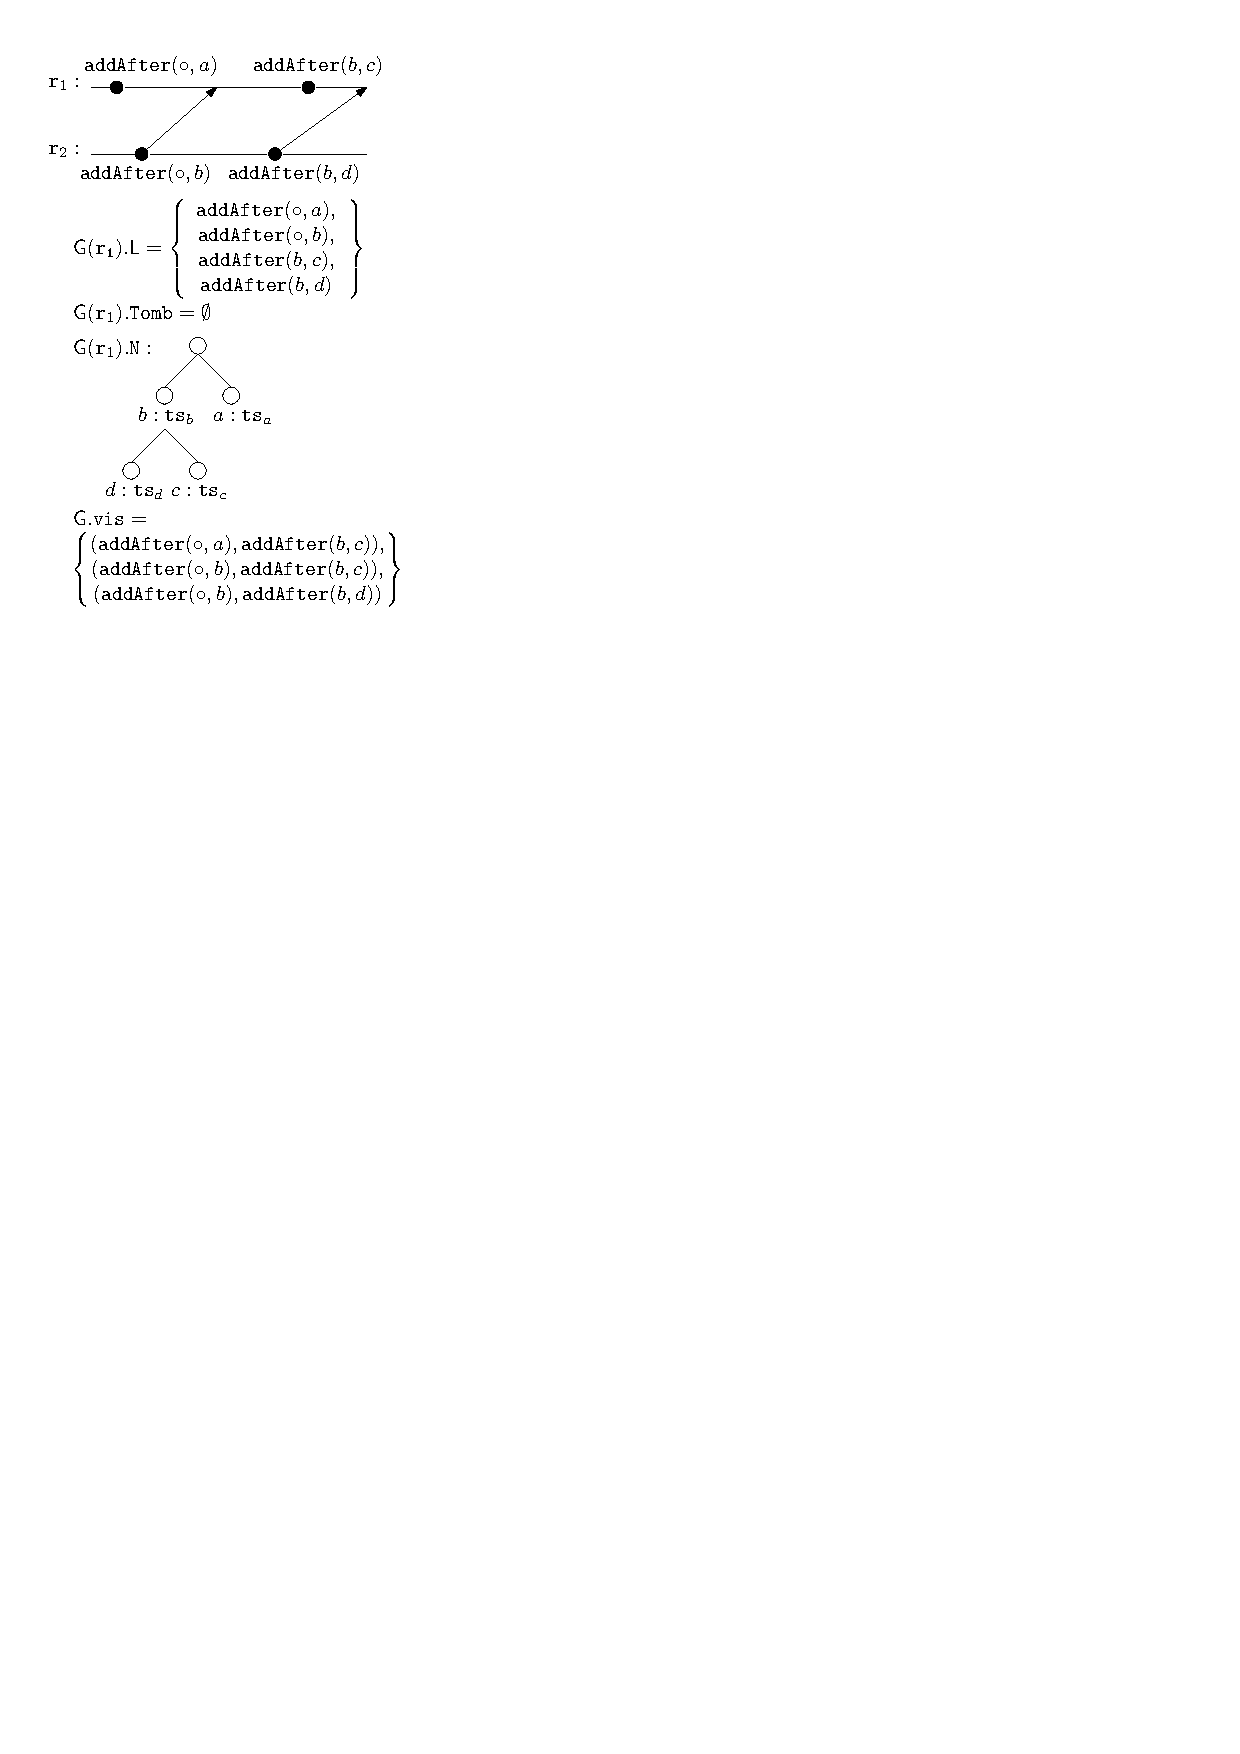
\includegraphics[scale=.7]{figures/LinRGA-2}
      \vspace{1cm}
    \caption{}
    \label{fig:rga-sem-2}
  \end{subfigure}
  \begin{subfigure}[!ht]{.3\linewidth}
    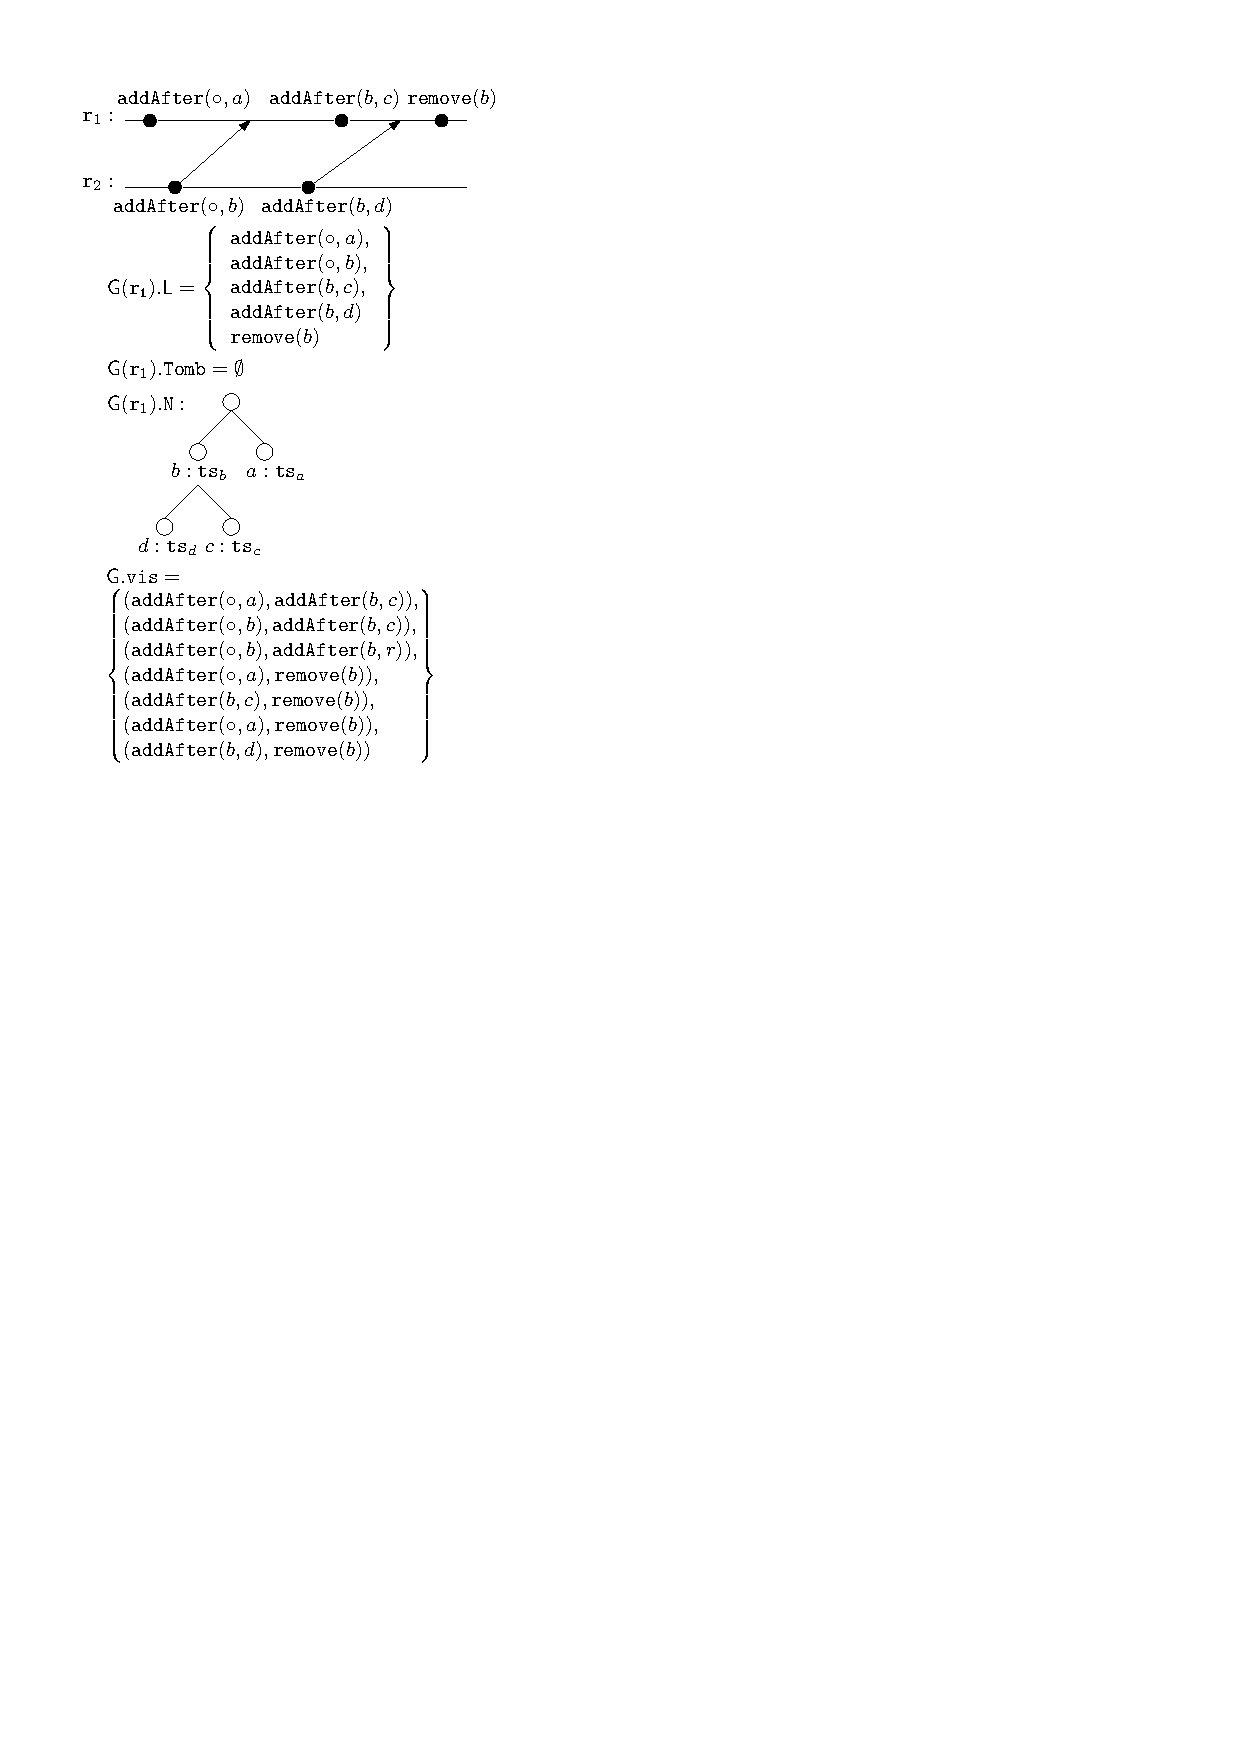
\includegraphics[scale=.7]{figures/LinRGA-3}
    \caption{}
    \label{fig:rga-sem-3}
  \end{subfigure}
  \caption{Example of the semantics of RGA }
  \label{fig:rga-sem}
\end{figure}

In the sequel it will be useful to distinguish query (or pure) methods
which do not modify the state from state-modifying methods, which we
shall call updates (or effectful).
%
We say that a method $\amethod\in\methods$ of object $\aobj\in \objs$
is a \emph{query} if it always results (by applying the {\tt atSource}
function $\atsource$) in an identity downstream $\effector$ (i.e.
$\delta(\sigma)=\sigma$ for all replica states
$\sigma$).\footnote{While we could have defined a semantics in which a
  read-only operation doesn't generate any downstream, we have preferred
  the current version for uniformity.}
We shall call an \emph{update} to any method $\amethod$ which is not a
query -- that is, whose effectors are not the identity function -- and
whose resulting downstream and return value do not depend on the
initial state $\astate$ of the origin replica.
That is, it's behavior is fully determined by its arguments.
More formally, assuming a functional equivalence relation $\equiv$
between downstreams that relates any two downstreams that have the same
effect (modulo the values of timestamps or unique identifiers)
$\amethod$ is called an update when
$\atsource(\sigma,\amethod,\argv)|_2 \equiv
\atsource(\sigma',\amethod,\argv)|_2$, for every $\argv\in\datadomain$
and two states $\sigma,\sigma'\in\Sigma$ (for a tuple $x$, $x|_k$
denotes the projection of $x$ on the $k$-th component).
A method $\amethod$ which is not a query nor an update is called a
\emph{query-update} (it generates a downstream which is not the
identity function, and whose effect depends on the local state of the
replica at which the invocation of $\amethod$ originated).
We denote by $\queries$, $\updates$, and $\queryupdates$, the sets of
operation labels $\alabelobjind{\argv}{\retv}{i,\ats}$ where $\amethod$
is a query, an update, or query-update respectively.
We shall call them query, update, and query-update labels,
respectively.
\fxwarning[nomargin, inline]{EXAMPLES OF QUERIES, UPDATES,
  QUERY-UPDATES.
  PROBABLY DISCUSSED ALREADY ALSO IN THE OVERVIEW.}

%Executions of an object $\aobj$ are defined as usual (as sequences of transitions in $\rightarrow$).
An execution of the object $\aobj$ is a sequence of transitions $\aglobalstate_0\xrightarrow{\aact_0}\aglobalstate_1\xrightarrow{\aact_1}\ldots$.
A \emph{trace} $\atrace$ is the sequence of actions $\aact_0\aact_1\ldots$ labeling the transitions of an execution.
The set of traces of an object $\aobj$ is denoted by $\traces(\aobj)$.
A \emph{history} is a pair $(\alabelset,\avisord)$ where
$\avisord\subseteq \alabelset\times\alabelset$ is an acyclic relation over the set of labels $\alabelset$.
% strict partial
%order over the set of labels $\alabelset$.
Given an execution $e$ ending in a global configuration $(\gstates,
\avisord, \downstreams)$, the \emph{history} of $e$, denoted by $\hist{e}$, is the pair
$(\labeldom{\avisord}, \avisord)$. Note that the relation $\avisord$ is a strict partial order in this case.
We will later allow a more general notion of history in order to deal
with object compositions (see Section~\ref{sec:compositionality}).
Also, the history of a trace $\atrace$, denoted by $\hist{\atrace}$,
is the history of the execution that corresponds to $\atrace$.
The set of histories $\histories(\aobj)$ of an object $\aobj$ is the
set of histories $h$ of an execution $e$ of $\aobj$.

\fxwarning[nomargin, inline]{EXAMPLE OF HISTORY OF AN EXECUTION.} {\color {red} CW: \figurename~\ref{fig:an example run of semantics} shows two steps of a history of RGA, and we can see how history grow in this example. Do I need to draw another figure start from initial global configuration?}

%\ce{Need to talk about read/updates}
%
%Without loss of generality we will consider that the methods in $\mathbb{M}$ can be separated in two disjoint sets of methods: $\mathbb{Q}$ query methods that has no influence on the ``abstract state'' and normally returns an observation of the ``abstract state'' , and $\mathbb{U}$ update methods that has influence on the ``abstract state''.

%
%A sequence $\aexec$ of operation labels is an execution of $\llbracket \aobj \rrbracket$, if there exists a global configuration $\aglobalstate = (\gstates, \avisord, \downstreams)$, such that $\aglobalstate_0 {\xrightarrow{ l }} \aglobalstate$. The history of $\aexec$ is a tuple $(\alabelset, \avisord)$, where $\alabelset$ is the set of labels of $l$. Let $\mathit{history}(\llbracket \aobj \rrbracket)$ be the set of histories of all executions of $\llbracket \aobj \rrbracket$. Then, $\aobj$ is \crdtlinearizable{}, if each of its history is, as stated by the following:
%
%
%
%\begin{definition}[Correctness of a CRDT Object]
%\label{definition:correctness of a CRDT object}
%A CRDT object $\aobj$ is \crdtlinearizable{} w.r.t a sequential specification \Spec{}, if each history of $\mathit{history}(\llbracket \aobj \rrbracket)$ is \crdtlinearizable{} w.r.t \Spec{}.
%\end{definition}
%

%\subsection{Histories}
%
%
%Firstly we will introduce the notion of \emph{histories} to represent
%abstractly the execution of a concrete client operating on an
%implementation of the data structure.
%
%Histories are composed of operation labels.
%We can now define execution \emph{histories}.
%
%\gpnote[nomargin, inline]{Maybe we have an overlap of IDs}
%% We assume a set $\aopid \in \opids$ to represent unique \emph{operation identifiers}.
%
%
%\begin{definition}[histories]
%  \label{definition:histories} An execution history is a tuple of the form
%  $(\alabelset, \avisord)$, where
%  \begin{enumerate}
%  \item $\alabelset$ is the set of labels representing the operations of
%    the execution,
%  % \item $\arepord \in (\alabelset \times \alabelset)$ is the
%  %   \emph{replica order}, a binary relation between the labels of the
%  %   execution, such that when restricted to labels of operations generated
%  %   by each single replica it is a total order, and it does not relate labels of
%  %   operations from different replicas, and
%  \item $\avisord \in (\alabelset \times \alabelset)$ is the
%    \emph{visibility order}, an \emph{acyclic partial order}
%    relation between the labels of the execution, such that if $(\alabel,
%    \alabel') \in \avisord$ then the operation corresponding to the label
%    $\alabel'$ witnessed in its execution the effects of the operation
%    with label $\alabel$.
%  \end{enumerate}
%\end{definition}

\subsection{Sequential Specifications}
\label{subsec:sequential specification}

\fxwarning[nomargin, inline]{INTRODUCE THIS SUBSECTION}

%\gp{We should add the specifications (even non-deterministic here.)}
\begin{definition}[Sequential Specification]
  \label{definition:sequential specification} A \emph{sequential
  specification} (specification, for short) $\Spec$ is a set of tuples $(\alabelset, \aseqord)$, where
  $\alabelset$ is a set of labels and
  $\aseqord$ is a sequence including all the labels in $\alabelset$.
\end{definition}

\gp{I'm changing the arrow because we use it in many places.}
To describe sequential specifications in a succinct way we will
provide an operational description.
To that end, we will associate to specifications a notion of abstract
state, which we shall generally denote by $\abstate$ and its domain
shall be denoted by $\abstates$.
Then, to each valid label $\alabel$ we will associate a transition
relation \;$\xrightharpoonup{\alabel}$\; which, given a state and provided
that the label can be applied into that state, produces a new abstract
state.
Hence, we denote by $\abstate \xrightharpoonup{\alabel}  \abstate'$
%$\absopsem{\abstate} = \abstate'$
the fact that the resulting state for label $\alabel$ with initial
abstract state $\abstate$ is $\abstate'$.
%
%To simplify our descriptions, we will use a shortcut notation for
%$\absopsem{\abstate} = \abstate'$ and will write it as:
%\[ \abstate \xrightharpoonup{\alabel}  \abstate' \]
In the specific case where the label $\alabel$ assumes a certain
precondition $\apre$ over the initial abstract state $\abstate$ we
will use Hoare-style preconditions and write
\[ \big(\abstate\ |\ \apre(\abstate)\big) \xrightharpoonup{\alabel}  \abstate' \]

A sequential specification then is the set of labels that are accepted
by the successive application of the transition relation starting from
some given initial state $\abstate_{0}$.

%A label is called \emph{read-only} if it doesn't change the abstract state, and a \emph{modifier} otherwise.
%The set of labels of a specification $\Spec$ is denoted by $\labelsspec\Spec$. The set of read-only, resp., modifier,
%labels of a specification $\Spec$ is denoted by $\labelsspecrd\Spec$, resp., $\labelsspecmod\Spec$.

% \fxwarning[nomargin, inline]{REWORK THESE EXAMPLES. DON'T WE NEED JUST
%   TWO EXAMPLES, RGA AND OR-SET ?}
% \gpnote[nomargin, inline]{Yes, I think so. Though it might be nice to
%   show more specs, since it kinda proves that they are easy to
%   read/write/understand.}

\gpwarning{Lots of rewriting to do here.}

Let us consider the specification of a very counter object, and then
the specifications of the RGA and OR-Set objects described above.

\begin{example}[Sequential Specification of a Counter]
\label{definition:sequential specification of counter}
The sequential specification $\mathit{counter}_s$ of counter is so
that $\abstates = \mathbb{Z}$, that is the state will be an integer,
and the transitions are given as follows:
\[
  \begin{array}[rcl]{rcl}
    k & \xrightharpoonup{\alabellong[\mathsf{inc}]{}{}} & k+1\\
    k & \xrightharpoonup{\alabellong[\mathsf{dec}]{}{}} & k-1\\
    k & \xrightharpoonup{\alabellong[\mathsf{read}]{}{k}} & k
  \end{array}
\]
% \begin{itemize}
% \setlength{\itemsep}{0.5pt}
% \item[-] $k \xrightharpoonup{\alabellong[\mathsf{inc}]{}{}} k+1$
% \item[-] $k \xrightharpoonup{\alabellong[\mathsf{dec}]{}{}} k-1$
% \item[-] $k \xrightharpoonup{\alabellong[\mathsf{read}]{}{k}} k$
% \end{itemize}
\end{example}


\begin{example}[Sequential Specification of RGA-like List
  (with $\mathtt{addAfter}$ method)]
  \label{definition:sequential specification of or-set}
  Each abstract state $\abstate = (l,T)$ contains a sequence $l$ of
  elements of a given type and a set $T$ of elements appearing in the
  list.
  The element $l$ is the list of all input values, whether already
  removed or not; while $T$ stores the removed values and is used as
  \emph{tombstone}.
  The sequential specification \gpnote*{Is this name used
    anywhere?}{$\mathit{listAft}_s$} of list with add-after interface is
  given with the transitions as follows:
  \[
    \begin{array}{rcl}
      \big(\ (l_1 \cdot a_k \cdot l_2,T\big)\ |\ a\text{ is fresh}\ \big)
      & \xrightharpoonup{\alabelshort[\mathtt{addAfter}]{a_k,a}}
      & (l_1 \cdot a_k \cdot a \cdot l_2,T)\\
      \big(\ (l,T)\ |\ a_k\ \text{occurs in}\ l\ \big)
      & \xrightharpoonup{\alabelshort[\mathtt{remove}]{a_k}}
      & (l,T \cup \{a_k\})\\
      (l,T)
      & \xrightharpoonup{\alabellong[\mathtt{read}]{}{s}{}}
      & (l,T)\
        \left[\begin{array}{c}
                 \text{with $s$ is obtained from $l$}\\
                 \text{by removing the values in $T$}
        \end{array}\right]
 \end{array}
  \]

  Method $\alabelshort[\mathtt{addAfter}]{a_k,a}$ puts $a$ immediately
  after $a_k$ in $l$, assuming that each value is put into list at
  most once.
  Method $\alabelshort[\mathtt{remove}]{a_k}$ adds $a_k$ into $T$,
  hence removing $a_k$ from the list for subsequent calls to the
  $\mathtt{read}$ method.
  Thus, $\alabellong[\mathtt{read}]{}{s}{}$ returns the list content
  excluding any element appearing in $T$.
  Assume that the initial value of list is $(\circ,\emptyset)$, and
  $\circ$ is never removed.
  When the context is clear, in $\ensuremath{\tt read}$ operation, we
  will omit $\circ$ in return value.
\end{example}

% {\color {red} CW: The sequential specification of OR-set and list with add-after interface}
\begin{example}[Sequential Specification of OR-Set]
\label{definition:sequential specification of or-set}
The query-update rewriting of OR-set is as follows: $\gamma( \alabelshort[{\tt remove}]{a} ) = ( \alabellong[{\tt readIds}]{a}{S}{}, \alabelshort[{\tt remove}]{a,S})$.


% \gpwarning{I still don't like the pairs for OR-Set}
Each abstract state $\abstate$ is a set of tuples $(a,id)$, where $a$
is a data and $id$ is a identifier. The sequential specification
$\mathit{OR-Set}_s$ of OR-Set is given by the transitions:
\[
  \begin{array}{rcl}
    \abstate
    & \xrightharpoonup{\alabellong[\mathtt{readIds}]{a}{S}{}}
    & \abstate\
      \begin{array}{c}
        [\text{with}\ S = \{ (a,id)\ \vert\ (a,id) \in \abstate\}]
      \end{array}\\
    \abstate &
               \xrightharpoonup{\alabelshort[\mathtt{remove}]{a,S}}
    & \abstate \setminus S \\
    \big(\ \abstate\ |\ \mathtt{id}\ \text{does not occur in } \abstate\ \big)
             & \xrightharpoonup{ \alabelshort[{\tt add}]{a,id} }
    & \abstate \cup \{ (a,\mathtt{id}) \}\\
    \abstate
    & \xrightharpoonup{\alabellong[\mathtt{read}]{a}{ S }{}}
    & \abstate\
      \begin{array}{c}
        [\text{with}\ S = \{ a\ \vert\ \exists\ \mathtt{id}, (a,\mathtt{id}) \in \abstate \}]
      \end{array}
  \end{array}
\]

Here $\alabellong[{\tt readIds}]{a}{S}{}$ returns the set of pairs with data $a$, $\alabelshort[{\tt remove}]{a,S}$ removes $S$ from the abstract state, $\alabelshort[{\tt add}]{a,id}$ puts $\{ (a,id) \}$ into the abstract state, and $\alabellong[{\tt read}]{}{S'}{}$ returns the value of the or-set.
\end{example}

\fxwarning[nomargin, inline]{TALK ABOUT SPECIFICATIONS OF A SET OF OBJECTS, OBTAINED AS A PRODUCT OF PER-OBJECT SPECIFICATIONS.}

\subsection{Definition of \CRDTLin{}}
\label{subsec:definition of distributed linearizability}

We now provide the definition of \crdtlin{} which characterizes histories of CRDT objects.
To simplify the presentation, we consider first the case where all the labels in the history are
either queries or updates (the case of query-updates is considered later in this section).
%
%To simplify the argument we will assume for the time being that all
%labels in a specification can be classified into update labels
%$\alabel_{up} \in \Updates$ and into $\alabel_{qr} \in \Queries$.
%Later we will extend the framework to consider query/update
%operations.
%
%We will generally assume that methods are predefined as either update
%or query, and labels are defined according to the method.
%In general however, given a specification in the operational style
%described above, we can identify a label as an update if in its
%specification the state before and after are different.
%Formally, if $\abstate \xrightarrow{\alabel} \abstate'$ belongs to $\Spec$
%and $\abstate \neq \abstate'$ we say that $\alabel$ is an update, and
%$\alabel \in \Updates$.\footnote{We assume that labels are
%  consistently update or query, should there be labels acting sometimes
%  as update and sometimes as only query, a simple renaming would suffice
%  to distinguish them.}
%A label is said to be a query if it is not an update.
%We will later add an additional case for query/update labels.
%
The intuition of our notion of \crdtlin{} is that there is a \emph{global} sequence
(or linearization) of the update operations in an execution which can
produce the state of \emph{each} replica when \emph{all} the updates are visible to them.
In intermediate steps, any replica state should be the result of applying a subsequence of updates
of this global sequence. This is because our semantical model allows replicas to see a subset of the updates
performed up to some moment.
%``explains'' the states of each replica,
%i.e., any state observed by any replica should be the result of applying a subsequence of updates
%in this sequence, and eventually, when all the updates are delivered at a replica~\footnote{Their corresponding downstreams are executed on that replica.}, its state is the result of applying this sequence of updates.
%%for update
%%operations there is a global linear sequence (or history) which can
%%produce the final state obtained by the execution.
%%In other words, any state observed by any replica should be the result
%%of a prefix of this sequential history.
%This notion is akin to Linearizability~\cite{HerlihyW90} when
%constrained to update-only operations.
%Evidently, this notion does not extend to query operations, since in
%our semantical model replicas can see a subset of the global updates
%performed at any moment, then we must allow for queries to read a
%sub-sequence of the updates in the global sequence mentioned above.
Therefore, each query should be justified by considering the
sub-sequence of the global sequence restricted to the updates that are
visible to that query.
To be precise:
%\gpnote*{We consider single-object only in this section} {A history is
%  single-object, if it contains operations of a single object.
%  A history is multi-object, if it contains operations of multiple
%  objects.}
%In the following we propose distributed linearizability for histories.
%\gpwarning*{}{We have to say that we distinguish query and update
%  labels, perhaps define formally (for queries the visibility is
%  important, updates change the state, but the visibility might not be
%  important.)}
%
%Before defining $\crdtlin{}$ it will be useful to present a definition
%of linearizability as given by Herlihy and Wing~\cite{HerlihyW90} but
%specialized for our notion of histories.
%We shall call this notion \HWLin{}.
%
%\begin{definition}[\HWLin{}]
%  A history $h = (\alabelset,\avisord)$ is related by \HWLin{}
%  w.r.t.
%  a sequential specification \Spec{}, if there exists a specification
%  history $(\alabelset, \aseqord) \in \Spec$,
%  called the \hwlinearization{} of $h$, where we require that $\aseqord$ be
%  consistent with $\avisord$ (i.e.
%  $(\aseqord \cup \avisord)^+$ is acyclic).
%  % Notice that this means that the visibility of operations in the
%  % \hwlinear{} history is exactly the prefix in $\aseqord$ up to that
%  % operation.
%\end{definition}
%
%This notion is too strong in general as we have shown in the examples
%of~\autoref{sec:CRDT implementations}.
%We shall relax this definition to accept histories where
%not all operations are seen by every query.
%
\begin{definition}
  \label{definition:ralinearizability1} A history $h =
  (\alabelset,\avisord)$ with $\alabelset\subseteq \queries\uplus\updates$ is \crdtlinearizable{} w.r.t. a
   sequential specification
%\gpnote*{First mention?}{deterministic}
  \Spec{}, if there exists a specification sequence
  $(\alabelset, \aseqord) \in \Spec{}$, called the
  \emph{\crdtlinearization{}} of $h$ -- where we remark that the set of labels
  are identical -- such that %
  % \gpwarning*{}{This definition has to be worked out again}
  \begin{enumerate}[(i)]
  \item \aseqord{} is consistent with  \avisord{}, that is: $(\avisord
    \cup \aseqord)^{+}$ is acyclic,
  \item the projection of $\aseqord$ to \emph{updates} is
    admitted by $\Spec$, i.e.
    $\aseqord\!\downarrow_{\updates} \in \Spec$, where we denote by
    $\aseqord\downarrow_{S}$ the restriction of the order $\aseqord$ to
    the set $S$, and
  \item for each query $\alabel_{\mathsf{qr}}\in \alabelset$, the subsequence of updates visible to $\alabel_{\mathsf{qr}}$ together with $\alabel_{\mathsf{qr}}$ is itself admitted by $\Spec$, i.e., $\aseqord\!\downarrow_{\avisord^{-1}(\alabel_{\mathsf{qr}})\cap \updates}\!\cdot\
    \alabel_{\mathsf{qr}} \in \Spec$.
\end{enumerate}
In this case we say that $(\alabelset, \aseqord)$ is an \emph{\crdtlinearization{}} of $h$ w.r.t. $\Spec{}$.
\end{definition}

In a nutshell, this definition requires that for a given
history, there exists a specification sequence such
that
\begin{inparaenum}[(i)]
\item the set of labels are the same and the order in the sequence is
  consistent with the visibility order of the history, that
\item when restricted to update operations -- that is all the updates --, the sequence belongs to
  the specification, and that
\item every query operations can be justified by the specification based only
  on the updates that precede it in the sequence and that are visible
  to it.
\end{inparaenum}

\fxwarning[nomargin, inline]{REFER TO AN EXAMPLE FROM THE OVERVIEW} {\color {red}CW: \figurename~\ref{fig:a history of RGA and its RA-linearization} gives a history of RGA and its linearization step by step.}

We now consider the case where histories include query-updates.
In such a case, we apply~\autoref{definition:ralinearizability1} on a
rewriting of the original history where each query-update is
decomposed into a label representing the query part and another label
representing the update part.
\gpnote*{Clarify this sentence. Not clear where the new labels come from}
{This rewriting may introduce new labels, which do not correspond to
original operations of the data type, but which have been extended to
be taken into account by the specification.
Also, other (update) operations of the object may be rewritten as
well.}
\fxwarning[nomargin, inline]{EXPLAIN THE OR-SET CASE.} {\color {red}CW: \figurename~\ref{fig:a history of OR-set, its update-query rewriting, and its RA-linearization} gives a history of OR-set, its query-update rewriting, and its \crdtlinearization{}.}

TODO MODIFY $\gamma$ BECAUSE IT MAY REWRITE UPDATES AS WELL. DO WE NEED TO REWRITE QUERIES ?

A mapping $\gamma:\labels\rightarrow \labels^{\leq 2}$, where $\labels^{\leq 2}$ is the set of labels and pairs of labels in $\labels$, is called a \emph{query-update rewriting}.
%Labels mapped by $\gamma$ to singletons preserve their query or update status
We assume that every query or update label is mapped by $\gamma$ to a singleton and that the $\gamma$ image of such a label preserves its status, i.e., $\gamma(\alabel)$ is a query, resp., update, whenever $\alabel$ is a query, resp., update. Also, query-updates labels $\alabel$ are mapped to pairs $\gamma(\alabel)=(\alabel_1,\alabel_2)$ where $\alabel_1$ is a query and $\alabel_2$ is an update. These assumptions are important when applying~\autoref{definition:ralinearizability1} on the rewriting of a history, since this definition relies on a partitioning of the labels into queries and updates.
%We say that $\gamma$ is \emph{consistent} with $\Spec$ when $\mathsf{image}(\gamma)\subseteq \labelsspec\Spec^{\leq 2}$ and for every label $\alabel$, if $\gamma(\alabel)=(\alabel_1,\alabel_2)$ then $\alabel_1$ is read-only and $\alabel_2$ is a modifier (of $\Spec$).
%For $\alabel\in \queryupdates$ and $\gamma(\alabel)=(\alabel_1,\alabel_2)$, the label $\alabel_1$ is considered a query and $\alabel_2$ an update.
For a history $h=(\alabelset,\avisord)$, its $\gamma$-rewriting is a
history $\gamma(h)=(\alabelset',\avisord')$ where
\begin{itemize}
\item $\alabelset'$ is obtained by replacing each label $\alabel$ in
  $\alabelset$ with $\gamma(\alabel)$ (a label may be replaced by two
  labels),
\item whenever a (query-update) label $\alabel$ is mapped by $\gamma$
  to a pair $(\alabel_1,\alabel_2)$ (i.e.
  $\gamma(\alabel)=(\alabel_1,\alabel_2)$), we have that the query is
  ordered before the update, formally $(\alabel_1,\alabel_2)\in \avisord'$,
\item $\avisord'$ preserves the order between labels which are
  mapped to singletons, and
  % whenever two labels are ordered by $\avisord$ and they are mapped
  % by $\gamma$ to singletons, then their $\gamma$-images remain
  % ordered in $\avisord'$. Similarly,
  for any query-update label $\alabel$ mapped to a pair
 $(\alabel_1,\alabel_2)$, the query $\alabel_1$ sees exactly the same
 set of operations as $\alabel$ and any operation which saw $\alabel$
 must see $\alabel_2$.
 Formally, whenever $(\alabel,\alabel')\in\avisord$ we have that
 $(\secondrep(\gamma(\alabel)),
 \firstrep(\gamma(\alabel')))\in\avisord'$, where for a label $\alabel$,
 $\firstrep(\gamma(\alabel))$ (resp., $\secondrep(\gamma(\alabel))$), is
 $\gamma(\alabel)$ when $\gamma(\alabel)$ is a singleton, or its first (resp.,
 second) projection when $\gamma(\alabel)$ is a pair.
\end{itemize}
The following definition
extends~\autoref{definition:ralinearizability1} to arbitrary histories
using the rewriting defined above.
% \gpnote[nomargin, inline]{I'd probably use $\Pi^*_i$ for the i-th
%   projection of a tuple, or the singleton.}

\begin{definition}[\CRDTLin{}]
  \label{definition:distributed linearizability} A history $h =
  (\alabelset,\avisord)$ is \crdtlinearizable{} w.r.t. a
   sequential specification
%\gpnote*{First mention?}{deterministic}
  \Spec{}, if there exists a query-update rewriting $\gamma$ such that $\gamma(h)$ is \crdtlinearizable{} w.r.t. \Spec{}.
\end{definition}


A set $H$ of histories is called \crdtlinearizable{} w.r.t a
sequential specification $\Spec$ when each history $h\in H$ is
\crdtlinearizable{} w.r.t.
$\Spec$.
A data type implementation is \crdtlinearizable{} w.r.t.
$\Spec$ if for any object $\aobj$ of the data type, the set
$\histories(\aobj)$ is linearizable w.r.t. $\Spec$.


\fxwarning[nomargin, inline]{MOVE THE FOLLOWING WHEN WE NEED IT (WHEN WE TALK ABOUT SOME NONDETERMINISTIC SPECIFICATION, E.G., WOOT)}

An important property of CRDT algorithms is \emph{convergence}.
Convergence means that all replicas will arrive to the same final
state when the same set of operations are applied to them.
For the moment we concentrate on specifications that are
\emph{deterministic}.
That is to say that for every label, the transition from a given
initial state can produce at most one final state.
We will later remove this restriction.
It is useful to remark that if the specification of a CRDT is
deterministic, then our definition of \crdtlin{} implies the
convergence of the data type, as formalized in the following lemma.

\begin{lemma}
\label{lemma:distributed linarizability implies convergence}
If a history $h$ is \crdtlinearizable{} w.r.t. a deterministic
sequential specification \Spec, then $h$ is convergent.
\end{lemma}









\forget{
\fxfatal[nomargin, inline]{Complete the others!}
\begin{example}[sequential specification of multi-value register]
\label{def:spec-MVR}
The sequential specification $\mathit{MVReg}_s$ of multi-value
register is given as follows: Let $\mathit{state}$ be a set and each
its element $(a,\mathit{id},f)$ is a tuple of a data $a$, an
identifier $\mathit{id} \in \mathbb{O}$, and a flag $f \in \{
\mathit{true},\mathit{false} \}$.
\begin{itemize}
\setlength{\itemsep}{0.5pt}
\item[-] $\{ \mathit{state} = S \}$ $(write(a),\mathit{id},S_1)$ $\{
  \mathit{state} = S[(b,\mathit{id}_1) \in S_2 : \mathit{false}] \cup
  \{ (a,id,\mathit{true}) \} \}$. Here $S_2 = \{ (b,\mathit{id}_1)
  \vert (b,\mathit{id}_1,\mathit{true}) \in S \wedge id \in S_1 \}$.
\item[-] $\{ \mathit{state} = S \wedge S_1 = \{ a \vert
  (a,\_,\mathit{true}) \in S \} \}$ $read() \Rightarrow S_1$ $\{
  \mathit{state} = S \}$.
\end{itemize}
\end{example}

\begin{example}[set and its sequential specification]
\label{definition:sequential specification of set}
A set has three methods: $\mathit{add}(a)$ inserts item $a$ into set;
$\mathit{rem}(a)$ removes $a$ from set; and $\mathit{read}$ returns
the set content.
% It implicitly assumes that each item being put into the set only
% once.
% Here we assume that when a item is removed, it will never be added
% again.
Here we assume that $\mathit{rem}$ will also be checked for
visibility.
The sequential specification $\mathit{set}_s$ of set is given as
follows:  Let $\mathit{state}$ be a set and each its element $(a,f)$
is a tuple of a data $a$ and a flag $f \in \{ \mathit{true},\mathit{false} \}$.
\begin{itemize}
\setlength{\itemsep}{0.5pt}
\item[-] $\{ \mathit{state} = S \wedge (a,\_) \notin S \}$
  $(\mathit{add}(a),\mathit{id})$ $\{ \mathit{state} = S \cup \{
  (a,\mathit{true}) \} \}$.
\item[-] $\{ \mathit{state} = S \wedge (a,\_) \in S \}$
  $(\mathit{add}(a),\mathit{id})$ $\{ \mathit{state} = S \}$.
\item[-] $\{ \mathit{state} = S \wedge (a,\_) \in S \}$
  $(\mathit{rem}(a))$ $\{ \mathit{state} = S[a: \mathit{false} \}$.
\item[-] $\{ \mathit{state} = S \wedge S_1 = \{a \vert
  (a,\mathit{true}) \in S \} \}$ $(\mathit{read}() \Rightarrow S_1)$
  $\{ \mathit{state} = S \}$.
\end{itemize}
\end{example}

%TODO TO MAKE IT MORE INTERESTING I ASSUME THAT REMOVE HAS A PRECONDITION: THE PAIRS REMOVED BY A REMOVE HAVE BEEN ADDED BEFORE

\begin{example}[OR-set and its sequential specification]
\label{def:specification-ORS}
OR-set is essential a multi-set: $\mathit{add}(a)$ inserts an item $a$
into multi-set; $\mathit{rem}(a)$ cancels only items $a$ that are
inserted by $\mathit{add}(a)$ operations visible to this remove
operation; $\mathit{read}$ returns the set of items in multi-set. A
value can be inserted multiple times.

The sequential specification $\mathit{OR}$-$\mathit{set}_s$ of OR-set
is given as follows: Let $\mathit{state}$ be a set and each its
element $(a,\mathit{id},f)$ is a tuple of a data $a$, an identifier
$\mathit{id}$, and a flag $f \in \{ \mathit{true},\mathit{false} \}$.
% In $((rem(a),\mathit{id}'),S_1)$, $S_1$ represents the operations
% visible to this remove operation.
\begin{itemize}
\setlength{\itemsep}{0.5pt}
\item[-] $\{ \mathit{state} = S  \wedge (\_,\mathit{id},\_) \notin S
  \}$ $(\mathit{add}(a),\mathit{id})$ $\{ \mathit{state} = S \cup \{
  (a,\mathit{id},\mathit{true}) \} \}$.
\item[-] $\{ \mathit{state} = S \wedge S_1 = \{ a \vert
  (a,\_,\mathit{true}) \in S \} \}$ $(\mathit{read}() \Rightarrow
  S_1)$ $\{ \mathit{state} = S \}$.
\item[-] $\{ \mathit{state} = S \wedge (a,\_,\_) \in S\}$
  $(rem(a),S_1)$ $\{ \mathit{state} = S[(a,\mathit{id}_1) \in S_2 :
  \mathit{false}] \}$. Here $S_2 = \{ (a,\mathit{id}_1) \vert
  (a,\mathit{id}_1,\mathit{true}) \in S \wedge id \in S_1 \}$.
\end{itemize}
\end{example}


\begin{example}[register and its sequential specification]
\label{def:spec-register}
A register has two methods: $\mathit{write}(a)$ writes $a$ into
register; $\mathit{read}$ returns the value of register. The
sequential specification $\mathit{reg}_s$ of register is given as
follows: Let $\mathit{state} \in \mathbb{D}$ be a value.
\begin{itemize}
\setlength{\itemsep}{0.5pt}
\item[-] $\{ \mathit{state} = a  \}$ $\mathit{write}(b)$ $\{
  \mathit{state} = b \}$.
\item[-] $\{ \mathit{state} = a \}$ $(\mathit{read}() \Rightarrow a)$
  $\{ \mathit{state} = a \}$.
\end{itemize}
\end{example}


\begin{example}[List with add-after interface]
\label{definition:spec-list-add-after}
Assume each item of the list is unique. A list has three methods:
$\mathit{add}(b,a)$ inserts item $b$ into the list at the position
immediately after that of item $a$; $\mathit{rem}(a)$ removes item $a$
from the list; and $\mathit{read}$ returns the list content. We assume
that the initial value of list is $(\circ,\mathit{true})$ and this
node can not be removed. We use the word ``add-after'' to emphasize
the method $\mathit{add}(b,a)$, which is different from the other list
interface that uses method $\mathit{add}(b,a,c)$.

The sequential specification $\mathit{list}_s^{\mathit{af}}$ of list
is given as follows: Let $\mathit{state}$ be a sequence, where each
item is a tuple $(a,\mathit{id},f)$ with data $a$, identifier
$\mathit{id}$ and flag $f \in \{ \mathit{true},\mathit{false} \}$.
Here $\mathit{af}$ represents add-after, and we use $l \uparrow_{S}$
to represent the projection of sequence $l$ into set $S$.
\begin{itemize}
\setlength{\itemsep}{0.5pt}
\item[-] $\{ \mathit{state} = (a_1,\mathit{id}_1,f_1) \cdot \ldots
  \cdot (a_n,\mathit{id}_n,f_n) \wedge k \leq n \wedge b \notin \{
  a_1, \ldots, a_n \} \wedge \mathit{id}_k \in S_1 \}$
  $(add(b,a_k),\mathit{id},S_1)$ $\{ \mathit{state} =
  (a_1,\mathit{id}_1,f_1) \cdot \ldots \cdot (a_k,\mathit{id}_k,f_k)
  \cdot (b,\mathit{id},\mathit{true}) \cdot
  (a_{k+1},\mathit{id}_{k+1},f_{k+1}) \cdot \ldots \cdot
  (a_n,\mathit{id}_n,f_n) \}$.
\item[-] $\{ \mathit{state} = (a_1,\mathit{id}_1,f_1) \cdot \ldots
  \cdot (a_n,\mathit{id}_n,f_n) \wedge k \leq n \wedge \mathit{id}_k
  \in S_1 \}$ $(rem(a_k),S_1)$ $\{ \mathit{state} =
  (a_1,\mathit{id}_1,f_1) \cdot \ldots \cdot
  (a_k,\mathit{id}_k,\mathit{false}) \cdot \ldots \cdot
  (a_n,\mathit{id}_n,f_n) \}$.
\item[-] $\{ \mathit{state} = (a_1,\mathit{id}_1,f_1) \cdot \ldots
  \cdot (a_n,\mathit{id}_n,f_n) \wedge S = \{ a \vert
  (a,\_,\mathit{true}) \in \mathit{state} \} \wedge l = a_1 \cdot
  \ldots \cdot a_n \uparrow_{S} \}$ $(read() \Rightarrow l)$ $\{
  \mathit{state} = (a_1,\mathit{id}_1,f_1) \cdot \ldots \cdot
  (a_n,\mathit{id}_n,f_n) \}$.
\end{itemize}
When the context is clear, in $\mathit{read}$ operation, we will omit
$\circ$.
\end{example}
}
%%% Local Variables:
%%% mode: latex
%%% TeX-master: "draft"
%%% End:
